\documentclass[dvipdfmx, tikz]{standalone}
\usepackage{tikz}
\usetikzlibrary{calc,decorations.pathreplacing,quotes,positioning,shapes,fit,arrows,backgrounds,tikzmark}

\begin{document}
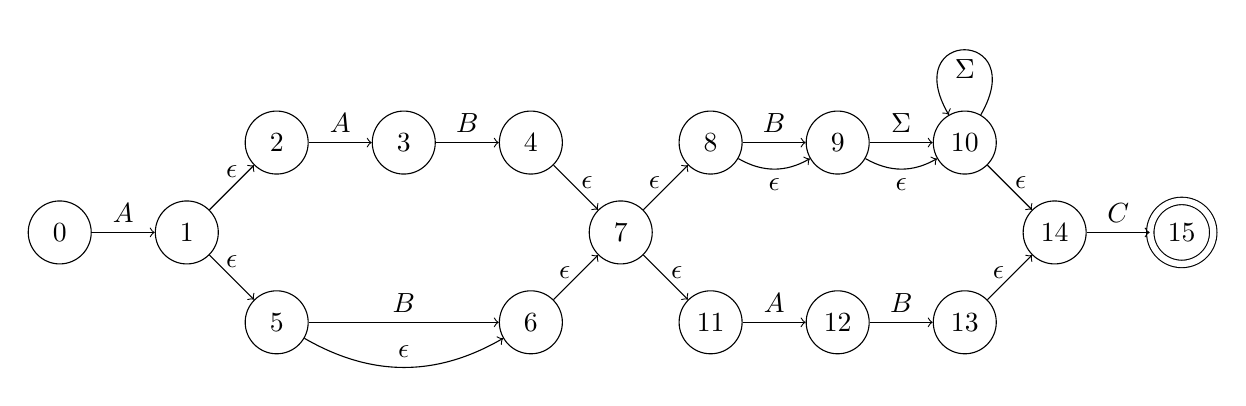
\begin{tikzpicture}[state/.style={circle, draw, minimum size=.8cm}, node distance=.8cm]
	\node(a0) [state] at (0,0) {$0$};
	\node(a1) [state, right =of a0] {$1$};
	\node(a2) [state, above right =of a1] {$2$};
	\node(a3) [state, right =of a2] {$3$};
	\node(a4) [state, right =of a3] {$4$};
	\node(a5) [state, below right =of a1] {$5$};
	\node(a7) [state, below right =of a4] {$7$};
	\node(a6) [state, below left = of a7] {$6$};
	\node(a8) [state, above right =of a7] {$8$};
	\node(a9) [state, right =of a8] {$9$};
	\node(a10) [state, right =of a9] {$10$};
	\node(a11) [state, below right =of a7] {$11$};
	\node(a12) [state, right =of a11] {$12$};
	\node(a13) [state, right =of a12] {$13$};
	\node(a14) [state, below right =of a10] {$14$};
	\node(a15) [state, double, double distance=.8mm, right =of a14] {$15$};

	\draw [->] (a0) to node[midway, above] {$A$} (a1) ;
	\draw [->] (a1) to node[midway, above] {$\epsilon$} (a2) ;
	\draw [->] (a1) to node[midway, above] {$\epsilon$} (a5) ;
	\draw [->] (a2) to node[midway, above] {$A$} (a3);
	\draw [->] (a3) to node[midway, above] {$B$} (a4);
	\draw [->] (a5) to node[midway, above] {$B$} (a6);
	\draw [->] (a5) to [bend right] node[midway, above] {$\epsilon$} (a6) ;
	\draw [->] (a4) to node[near end, above] {$\epsilon$} (a7) ;
	\draw [->] (a6) to node[near start, above] {$\epsilon$} (a7) ;
	\draw [->] (a7) to node[near start, above] {$\epsilon$} (a8) ;
	\draw [->] (a7) to node[near end, above] {$\epsilon$} (a11) ;
	\draw [->] (a8) to node[midway, above] {$B$} (a9) ;
	\draw [->] (a9) to node[midway, above] {$\Sigma$} (a10) ;
	\draw [->] (a8) to [bend right] node[midway, below] {$\epsilon$} (a9) ;
	\draw [->] (a9) to [bend right] node[midway, below] {$\epsilon$} (a10) ;
	\draw [->] (a10) to [out=60, in=120, looseness=8] node[midway, below] {$\Sigma$} (a10) ;
	\draw [->] (a11) to node[midway, above] {$A$} (a12) ;
	\draw [->] (a12) to node[midway, above] {$B$} (a13) ;
	\draw [->] (a10) to node[near end, above] {$\epsilon$} (a14) ;
	\draw [->] (a13) to node[near start, above] {$\epsilon$} (a14) ;
	\draw [->] (a14) to node[midway, above] {$C$} (a15) ;
\end{tikzpicture}
\end{document}
